\subsection{Periodicity Tasks}\label{synth-benchmark:periodicity}


We introduce a family of synthetic tasks designed to evaluate the ability of TGL  methods to learn periodic structure through time. Solving these tasks requires \emph{counting} and \emph{memorization} capabilities, under both deterministic and stochastic settings.


% \begin{figure}[ht]

\begin{figure}[ht]
    \centering
    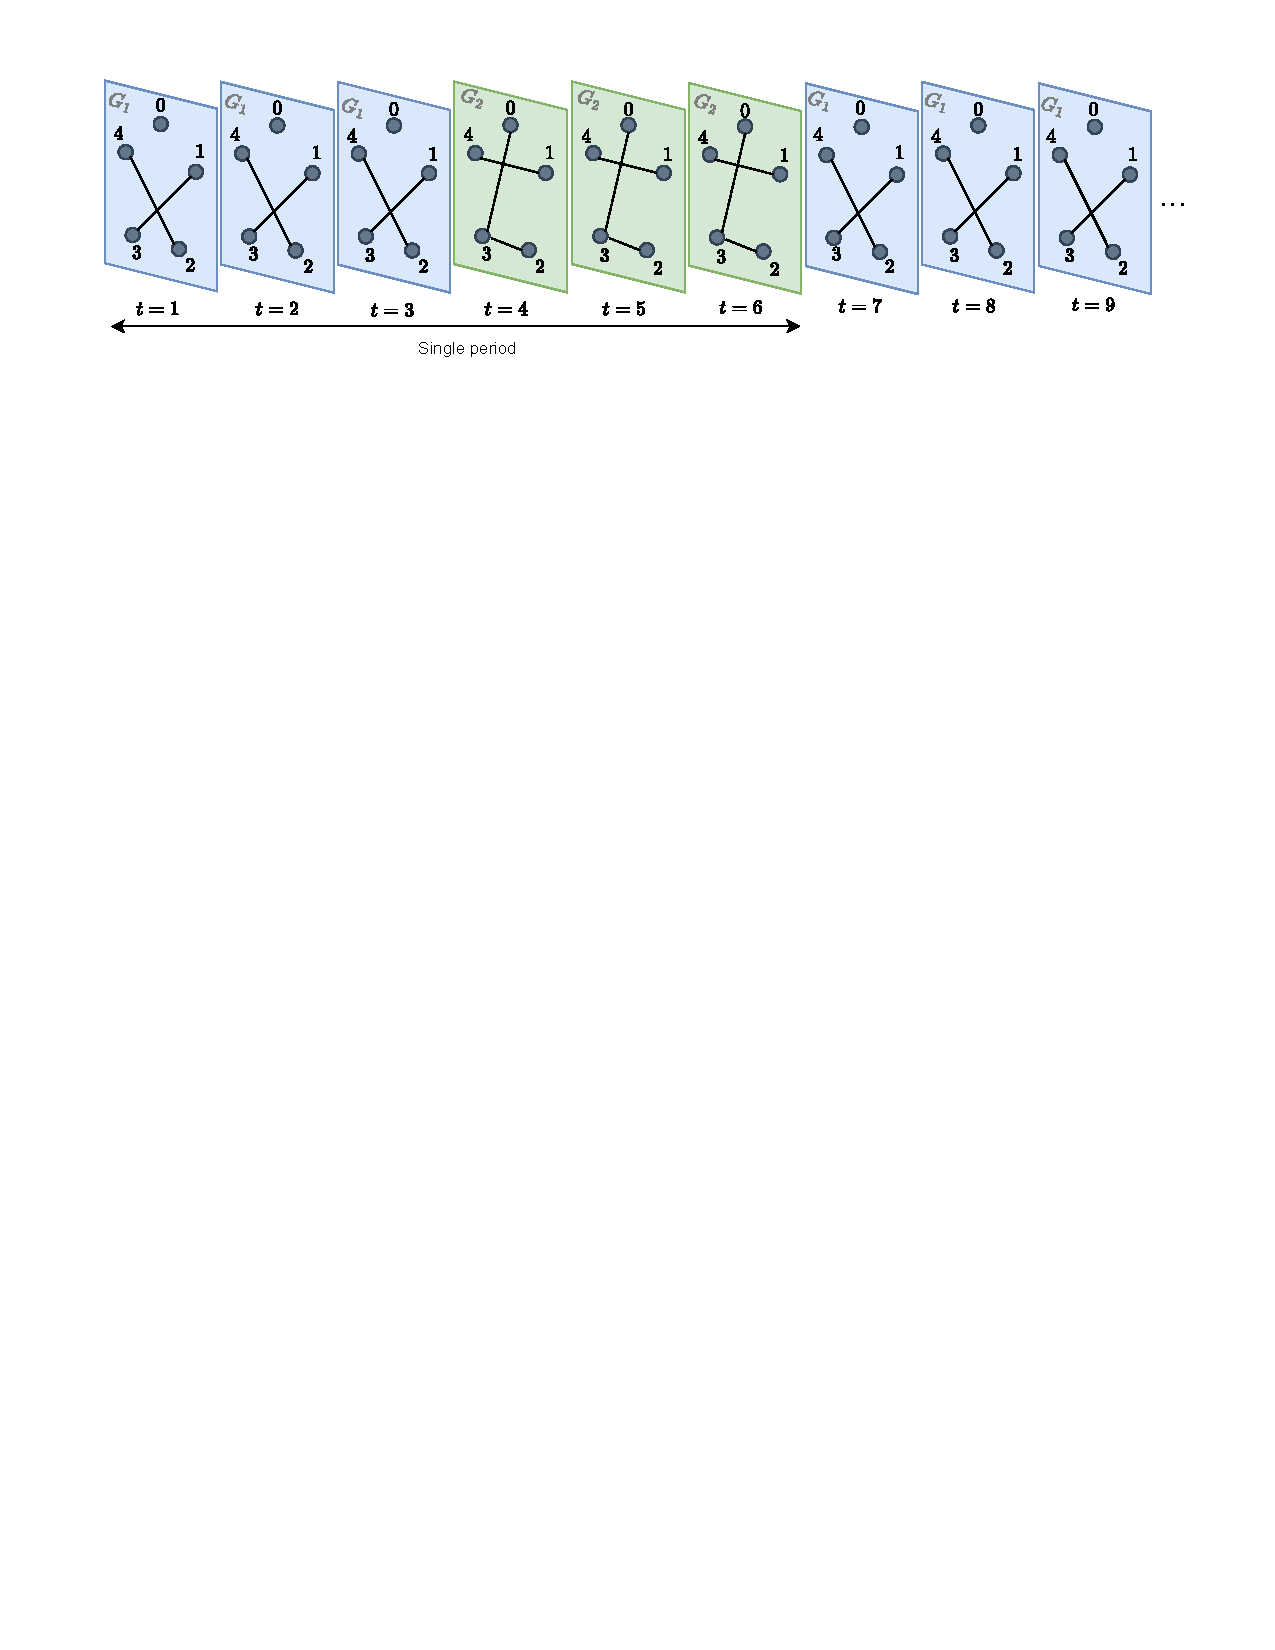
\includegraphics[width=\linewidth, height=8em, keepaspectratio]{figs/periodicity/Fixed_ER/(2, 3)_dataset.pdf}
    \caption{A periodic task in $\Pdet{k=2,n=3}$ containing two unique snapshots, each repeated three times within a single period. }
    \label{fig:periodicity}
\end{figure}


\begin{definition}[Periodicity Tasks]
Let $k, n \in \mathbb{N}$. The task families $\Pdet{k,n}$ and $\Psto{k,n}$ are defined based on a repeating pattern $p$ where each integer $i \in \{1,\dots,k\}$ appears $n$ consecutive times before cycling. At each time step $t$, let $i_t = (\lfloor t/n\rfloor \mod k) + 1$.
In $\Pdet{k,n}$, the dynamic graph $\mathcal{G} = G_1, G_2, \dots$ is a periodic sequence alternating between $k$ fixed static graphs $G_1, \dots, G_k$, i.e., $G_t = G_{i_t}$.
In $\Psto{k,n}$, each $G_t$ is sampled from one of $k$ distributions $D_1, \dots, D_k$ over static graphs (e.g., Erd\H{o}s-Rényi~(ER)~\cite{erdos1960evolution}, Stochastic Block Model~(SBM)~\cite{holland1983stochastic}), with $G_t \sim D_{i_t}$. The resulting sequence is stochastic, but the distribution pattern follows the  periodic structure of $\Pdet{k,n}$.
\end{definition}

For example, a task in $\Pdet{k=3,n=2}$  will correspond to a dynamic graph $ G_1,G_1,G_2,G_2,$ $G_3,G_3,G_1,G_1,$..., where $G_1,G_2,G_3$ are static graphs. A task  illustration is shown in $\Pdet{k,n}$ is shown in Figure~\ref{fig:periodicity}.



\textbf{Task objectives.}
Tasks in $\Pdet{k,n}$ test the counting and memory capacity of TGL methods. The parameter $k$ controls the length of the pattern and thus the memory demand, while $n$ governs how long each graph is repeated and tests the model's ability to count. For instance, solving a task in $\Pdet{2,n}$ requires counting up to $n$ before switching graphs, while solving a task in $\Pdet{k,1}$ requires memorizing $k$ static graphs. Tasks in $\Psto{k,n}$ introduce stochasticity, requiring models to reason over distributions rather than fixed structures, increasing the complexity while retaining the same periodic structure. 
%Detailed dataset statistics of the dataset we generated for these tasks can be found in \Cref{appendix:periodicity-deterministic-stats}.


\begin{figure}
    \centering
    \begin{subfigure}[b]{0.3\textwidth}
        \centering
        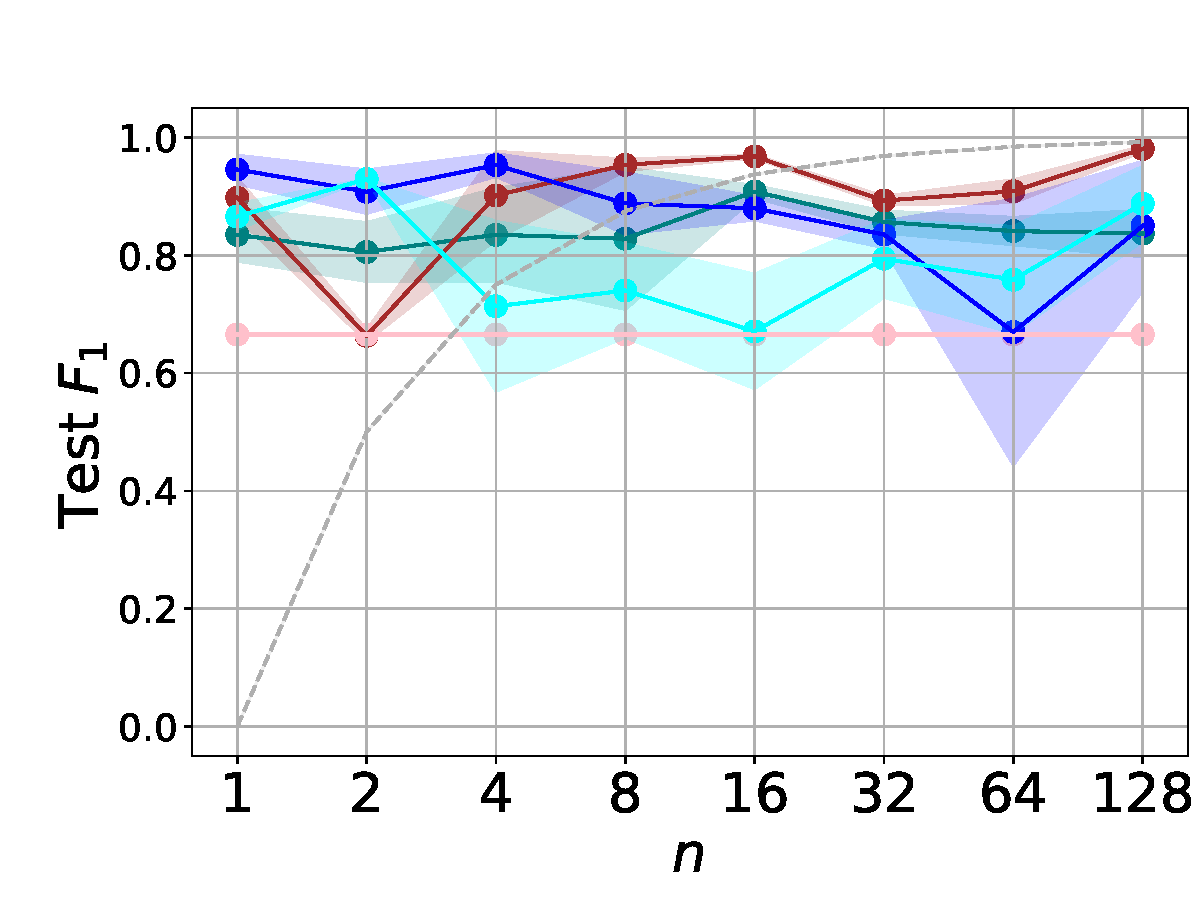
\includegraphics[width=\linewidth,trim={0 2.25cm 0 0},clip]{figs/periodicity/Fixed_ER/(2, n)CTDG_Test $F_1$.pdf}      
        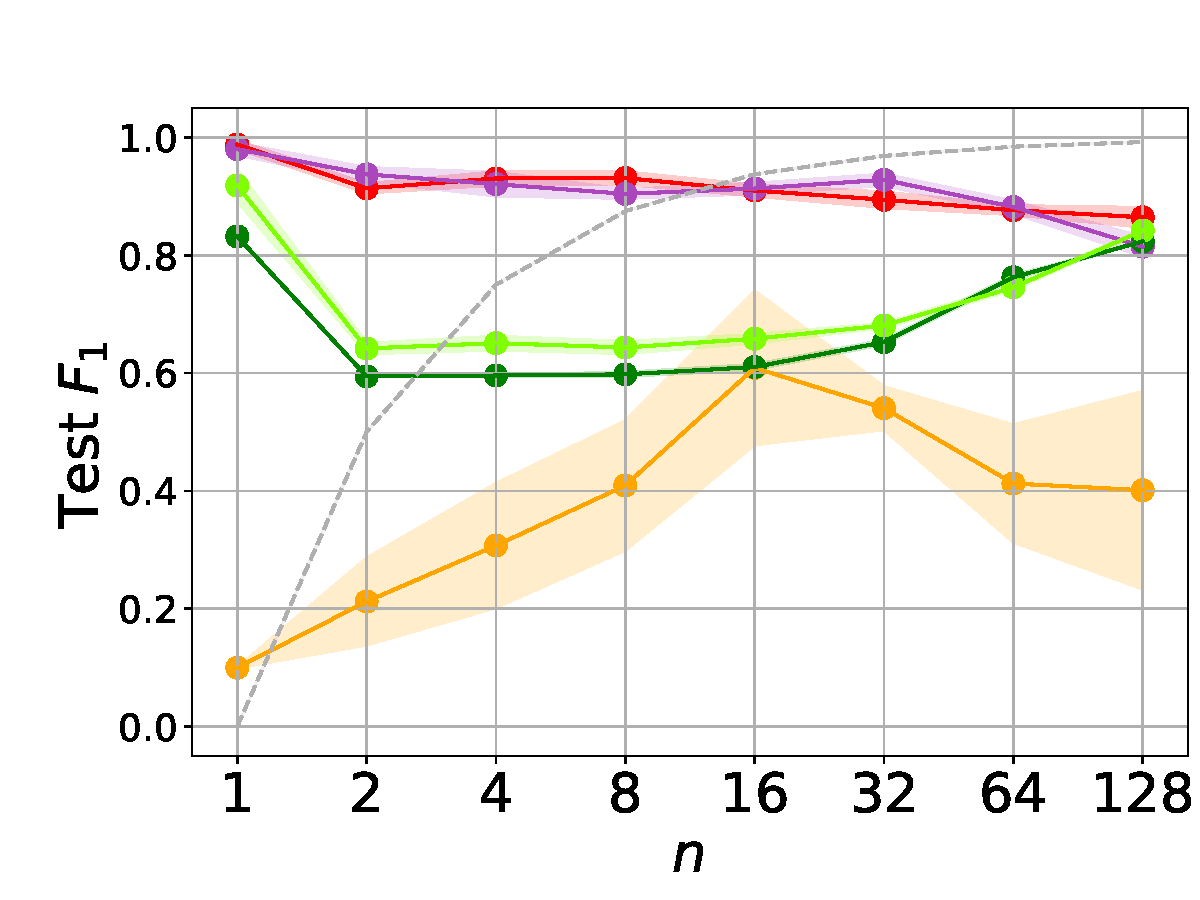
\includegraphics[width=\linewidth,trim={0 0 0 1.2cm },clip]{figs/periodicity/Fixed_ER/(2, n)DTDG_Test $F_1$.pdf}
        \caption{$\Pdet{2,n}$ - All time steps.}
        \label{fig:dtdg_(2,n)_allsteps}
    \end{subfigure}
    \begin{subfigure}[b]{0.3\textwidth}
        \centering
        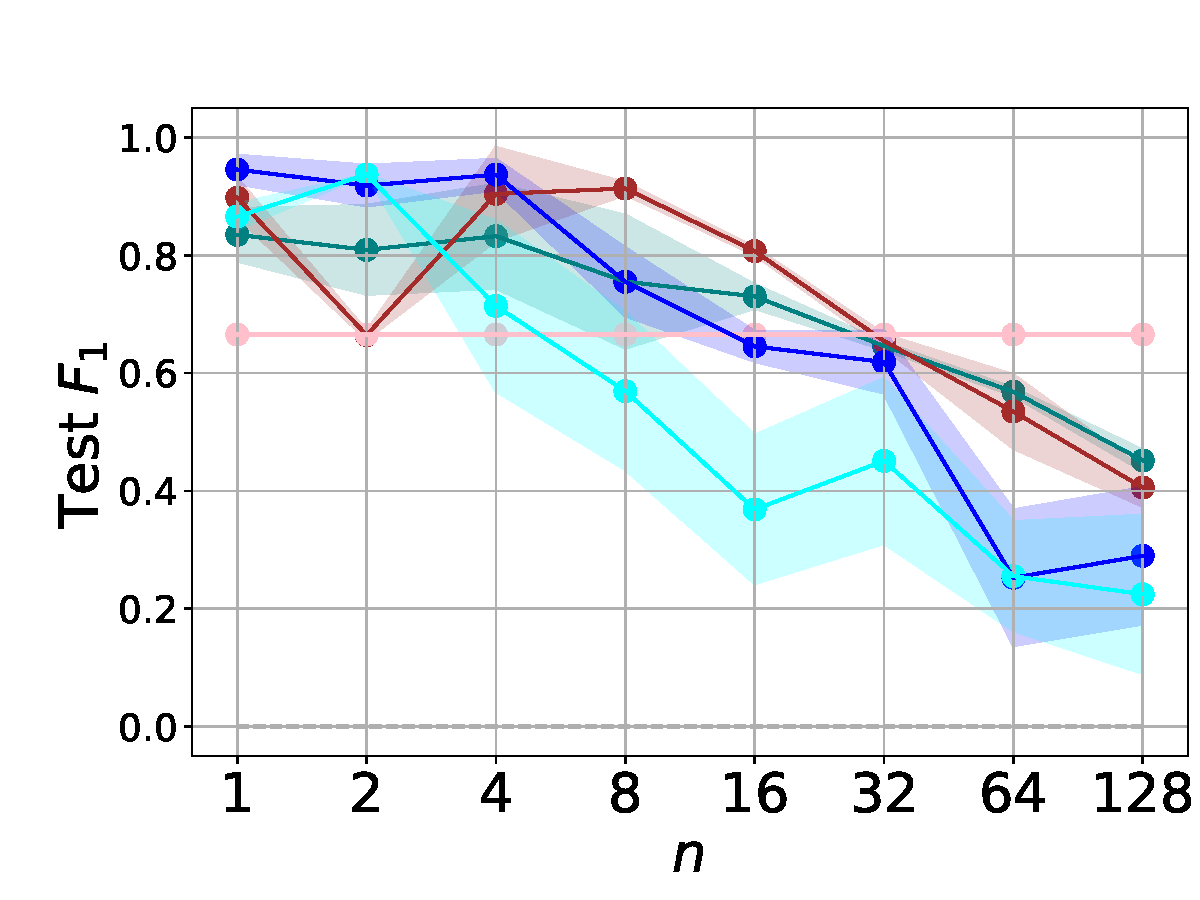
\includegraphics[width=\linewidth,trim={0 2.25cm 0 0},clip]{figs/periodicity/Fixed_ER/change_point/(2, n)CTDG_CP_Test $F_1$.pdf}
        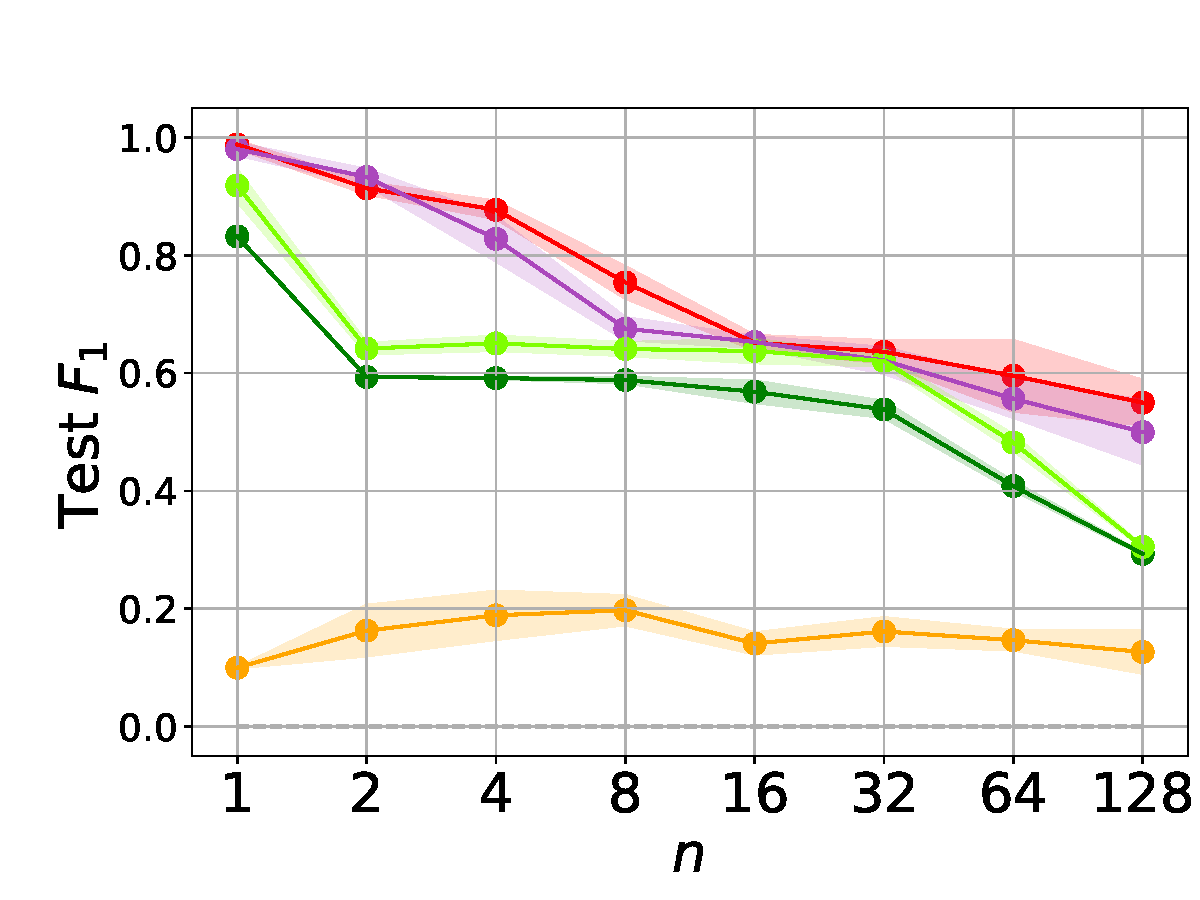
\includegraphics[width=\linewidth,trim={0 0 0 1.2cm },clip]{figs/periodicity/Fixed_ER/change_point/(2, n)DTDG_CP_Test $F_1$.pdf}
        \caption{ $\Pdet{2,n}$ - Change points.}
        \label{fig:dtdg_(2,n)_changepoints}
    \end{subfigure}
    \begin{subfigure}[b]{0.3\textwidth}
        \centering
        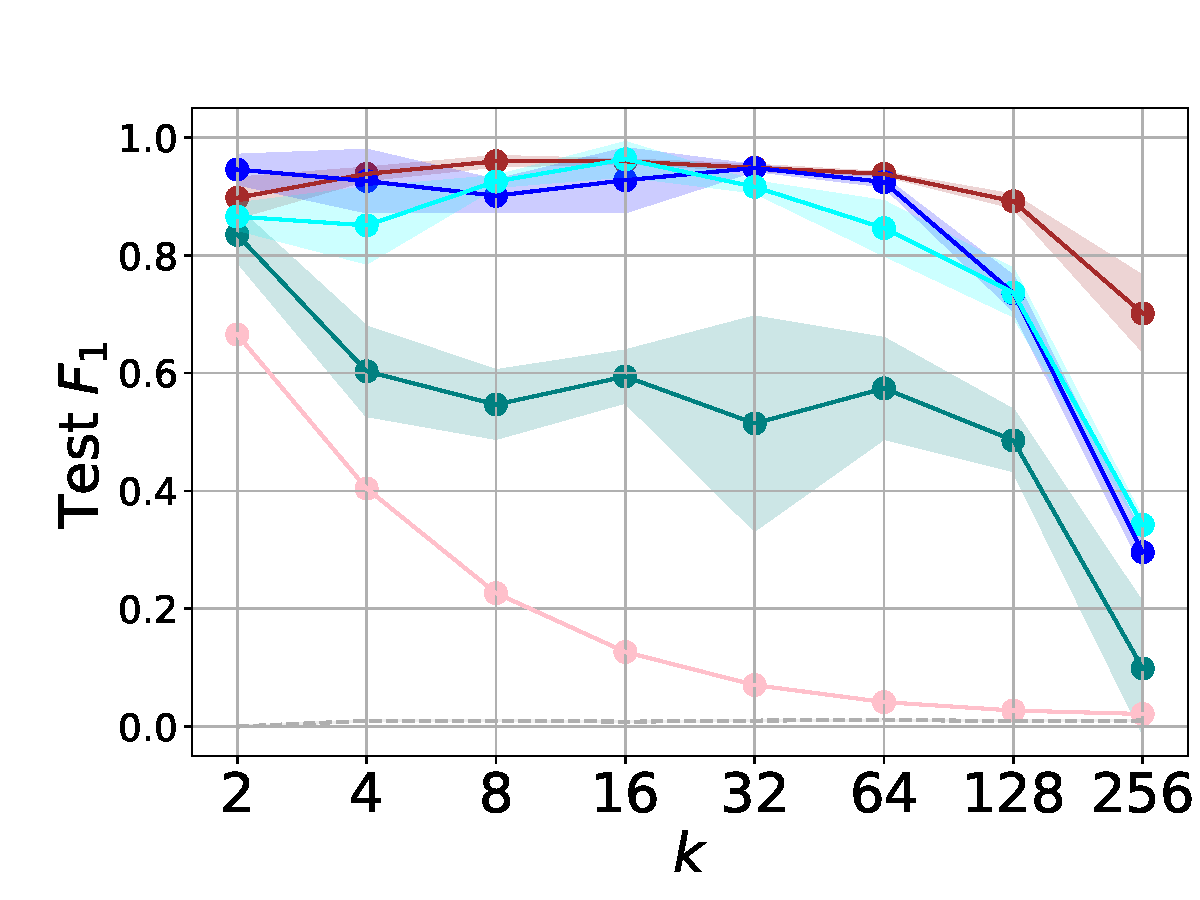
\includegraphics[width=\linewidth,trim={0 2.25cm 0 0},clip]{figs/periodicity/Fixed_ER/(k, 1)CTDG_Test $F_1$.pdf}
        
        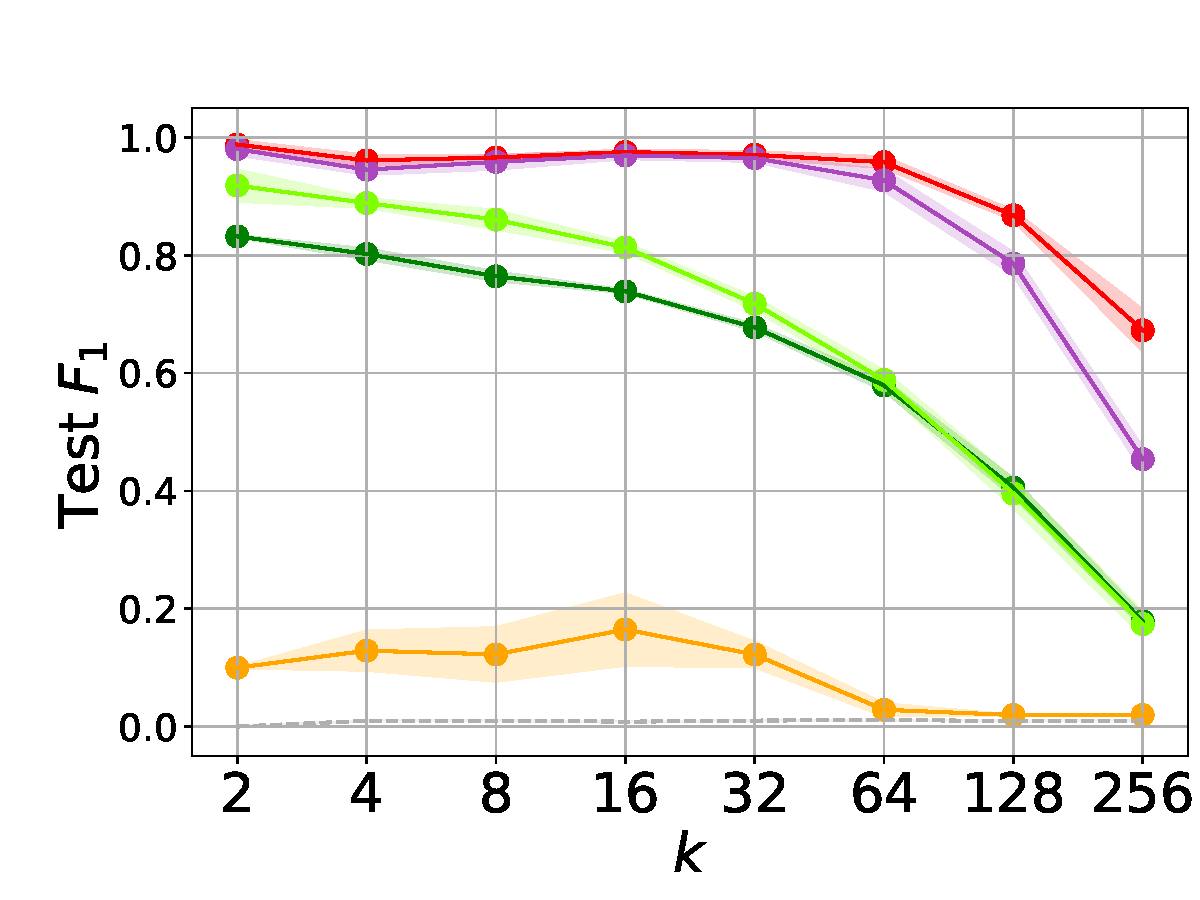
\includegraphics[width=\linewidth,trim={0 0 0 1.2cm },clip]{figs/periodicity/Fixed_ER/(k, 1)DTDG_Test $F_1$.pdf}
        \caption{$\Pdet{k, 1}$ - All time steps.}
        \label{fig:dtdg_(k, 1)}
    \end{subfigure}
    \begin{subfigure}[b]{0.08\textwidth}
        \centering
        \raisebox{14mm}{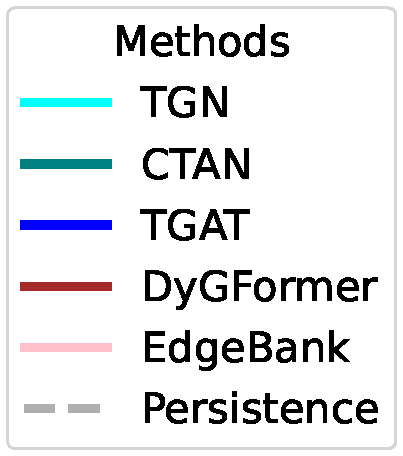
\includegraphics[width=\linewidth]{figs/legends/CTDG w persistence.pdf}}
        
        \raisebox{14mm}{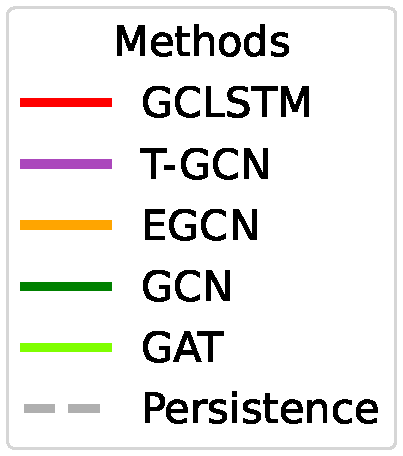
\includegraphics[width=\linewidth]{figs/legends/DTDG w persistence.pdf}}
    \end{subfigure}
    
    \caption{
    Performance of CTDG methods (top row) and DTDG methods (bottom row) on the deterministic periodicity tasks.
    %$\Pdet{2, n}$~(left and center) and $\Pdet{k, 1}$~(right). 
    }
    \label{fig:det_periodic_overall}
\end{figure}




% \at{The following feels out of place?} \ah{I will try rephrasing.}
% \ah{we use $n$ for number of nodes and number of repetions?? notation overload. Do we even need to explain the graph construction for every task?}\gr{No, number of nodes should be $N$}

\looseness-1 \textbf{Can TGNNs count?} To evaluate the counting ability of TGNNs, we construct tasks in $\Pdet{k,n}$ and the graphs are sampled from the Erdős-Rényi~(ER) model~\citep{erdos1960evolution}~(100 nodes and edge probability 0.01). We set $k = 2$ and vary $n$. The increase in $n$ corresponds to the increase in task difficulty as models are required to count longer sequences. 
Model performance on these $\Pdet{2,n}$ tasks for values of $n$ ranging from 1 to 128 is presented in \Cref{fig:det_periodic_overall}. We report the $F_1$ score for dynamic link prediction, evaluated in two crucial ways: first, over all timesteps (left plot), and second, exclusively at change points (center plot). 
Since models repeating the previous timestep can perform well for large $n$, we report $F_1$ both over all timesteps (left) and at change points only (center), where the active graph switches, i.e., $t = n+1, 2n+1, \cdots$. A high score at change points indicates true counting and pattern understanding, whereas a low score, even with good overall performance, suggests the model is merely exploiting continuity rather than reasoning about the period length.

\looseness-1 The results reveal distinct behaviors across different TGNN families. Averaging $F_1$ performance across all timesteps and among CTDG models, TGAT performs well for small $n$, while DyGFormer demonstrates more consistent performance at larger $n$. For DTDG methods, T-GCN and GC-LSTM are strongest overall. Interestingly, EvolveGCN performs worse than the static graph learning methods, GCN and GAT, which lack any temporal processing mechanisms, underscoring the difficulty these simple periodic patterns can pose for current TGNNs. EdgeBank remains constant for all $n$, always predicting the union of both graphs, making its output insensitive to $n$. The persistence baseline improves over all timesteps as $n$ increases by simply copying the previous snapshot, but scores zero at change points.

\looseness-1 A key observation, evident when comparing performance over all timesteps vs. at change points (\Cref{fig:det_periodic_overall}), is that as $n$ grows, many models increasingly rely on repetition rather than explicit counting. While their overall scores might remain high or even improve for larger $n$ (due to successfully predicting links during the long static phases), their performance at change points often degrades or fails to improve proportionally. At $n = 32$, EdgeBank even starts to outperform all TGNNs. This divergence suggests that current TGNNs struggle to robustly count long sequences and instead learn a simpler heuristic reminiscent of persistence. % Further per-timestep analysis supporting this trend is provided in Appendix~\ref{appendix:pertimesteps_counting}.

\looseness-1 \textbf{How much can TGNNs memorize?} To evaluate the memorization capabilities of TGNNs, we fix $n = 1$ and vary $k$. The challenge, therefore, scales directly with $k$: as more unique graph structures are introduced, models must maintain a larger and more distinct set of representations in their memory to correctly predict links at each timestep. \label{seq:memorize}

\looseness-1 Figure~\ref{fig:det_periodic_overall} (right) shows results on $\Pdet{k, 1}$ for values of $k$ ranging from 2 to 256. As expected, Edgebank steadily degrades to zero performance at $k = 256$, eventually defaulting to predicting each snapshot as a clique. However, all TGNN models show a gradual decline as $k$ increases. GCLSTM and DyGFormer consistently perform best, showing strong memorization of diverse patterns. T-GCN, TGN, and TGAT remain robust up to $k = 128$, but drop sharply at $k = 256$, suggesting that current models that we have tested reached their maximum capacity for memorizing at the mentioned dropping points.
% -- suggesting their capacity to distinguish and recall a large set of unique graph states is more abruptly exhausted. 

\looseness-1 On a somewhat surprising contrast, TGNNs such as CTAN (CTDG) and  EvolveGCN (DTDG) struggle significantly more as the number of unique graphs increases. CTAN's performance, for instance, begins to degrade considerably after $k=64$.
Notably, both these methods are often outperformed by static GNNs like GCN and GAT --which exhibit a more gradual decline. Their relative success might indicate that for tasks dominated by the need to memorize many distinct states, an ineffective temporal mechanism can be more detrimental than no temporal mechanism at all.
% In this setting, a model must (1) identify which of $G_1, \dots, G_k$ the current snapshot $G_t$ corresponds to, and (2) memorize the sequence to predict the next graph in the $k$-periodic cycle. 

% % \looseness-1
% To probe the \textit{memorization} capabilities of TGNNs, we can conversely vary $k$ and fix $n = 1$. In this setting, a given model needs to be able to 1) determine which of $G_1 \dots G_k$ is some $G_t$ equal to and 2) \textit{memorize} events in the past to determine what comes next in $k$-length periodic sequence.
% As $k$ increases, the task increases in difficulty as it requires the model to memorize a longer sequence of past events. 

% Figure~\ref{fig:det_periodic_overall}~(right) shows the performance of all methods on the task $\Pdet{k, 1}$ datasets for values of $k$ ranging from 2 to 256. All methods gradually lose memorization ability as $k$ increases. GCLSTM and DyGFormer consistently achieve the highest performance across all values of $k$, demonstrating strong memorization of diverse patterns. T-GCN, TGN, and TGAT remain robust up to $k = 128$, but show a significant drop at $k = 256$. Surprisingly, CTAN and  EvolveGCN underperform even compared to static methods like GCN and GAT, which ignore temporal information. As expected, Edgebank performance degrades steadily, reaching zero for $\Pdet{256, 1}$, eventually defaulting to predicting each snapshot as a clique at higher $k$.



% Note that we did not include $k = 1$ as it is a degenerate case with only one graph type in the deterministic case or one distribution in the stochastic case. 

\looseness-1 \textbf{Can TGNNs learn stochastic periodic structures?} Lastly, we examine how the models' memorization abilities extend to a probabilistic setting, where the periodic structure is not explicitly observable but arises from a stochastic process. 
% latent generative process. To this end, we generate tasks in the $\Psto{k,1}$ setting for $k$ values ranging from 2 to 64.
Each of the $k$ distributions follows a Stochastic Block Model (SBM) over 100 nodes divided into 3 communities. While all SBM distributions share the same intra- and inter-community edge probabilities, they differ in their community structures
%~(see Appendix~\ref{appendix:periodicity_stochastic_design} for details)
.
The inter-community edge probability is fixed at 0.01, while the intra-community edge probability $p$ takes values 0.9 and 0.5.
%The inter-community edge probability is fixed at 0.01, meaning an edge between nodes in different communities appears with probability 0.01. We consider two values for the intra-community edge probability $p$, where an edge between nodes in the same community appears with probability $p$: specifically, $p = 0.9$ and $p = 0.5$. %For each value of $k$, models are trained on $40k$ snapshots, validated on $4k$ and tested on $4k$ snapshots.

Figure~\ref{fig:(K,1)_overall_sto} presents the performance of TGL models. As expected, model performance generally decreases as $k$ increases, reflecting the growing difficulty of memorizing a larger number of stochastic patterns. GCLSTM consistently achieves the highest performance across both values of $p$, demonstrating strong memorization capabilities even in noisy environments, where TGAT is the second top-performing method. While T-GCN also performs strongly in the easiest setting $p=0.9$~(left), it struggles in the noisier setting~(right), falling behind TGAT and TGN. Overall, model performance decreases under a lower intra-community density ($p = 0.5$), 
indicating that increased stochasticity further challenges memorization, as expected. However, compared to the deterministic case, static baselines (GCN and GAT) underperform TGNNs, highlighting the effectiveness of temporal modeling in capturing latent periodic structures in dynamic graphs.

\begin{figure}
    % (k, 1) CTDG
    \centering
        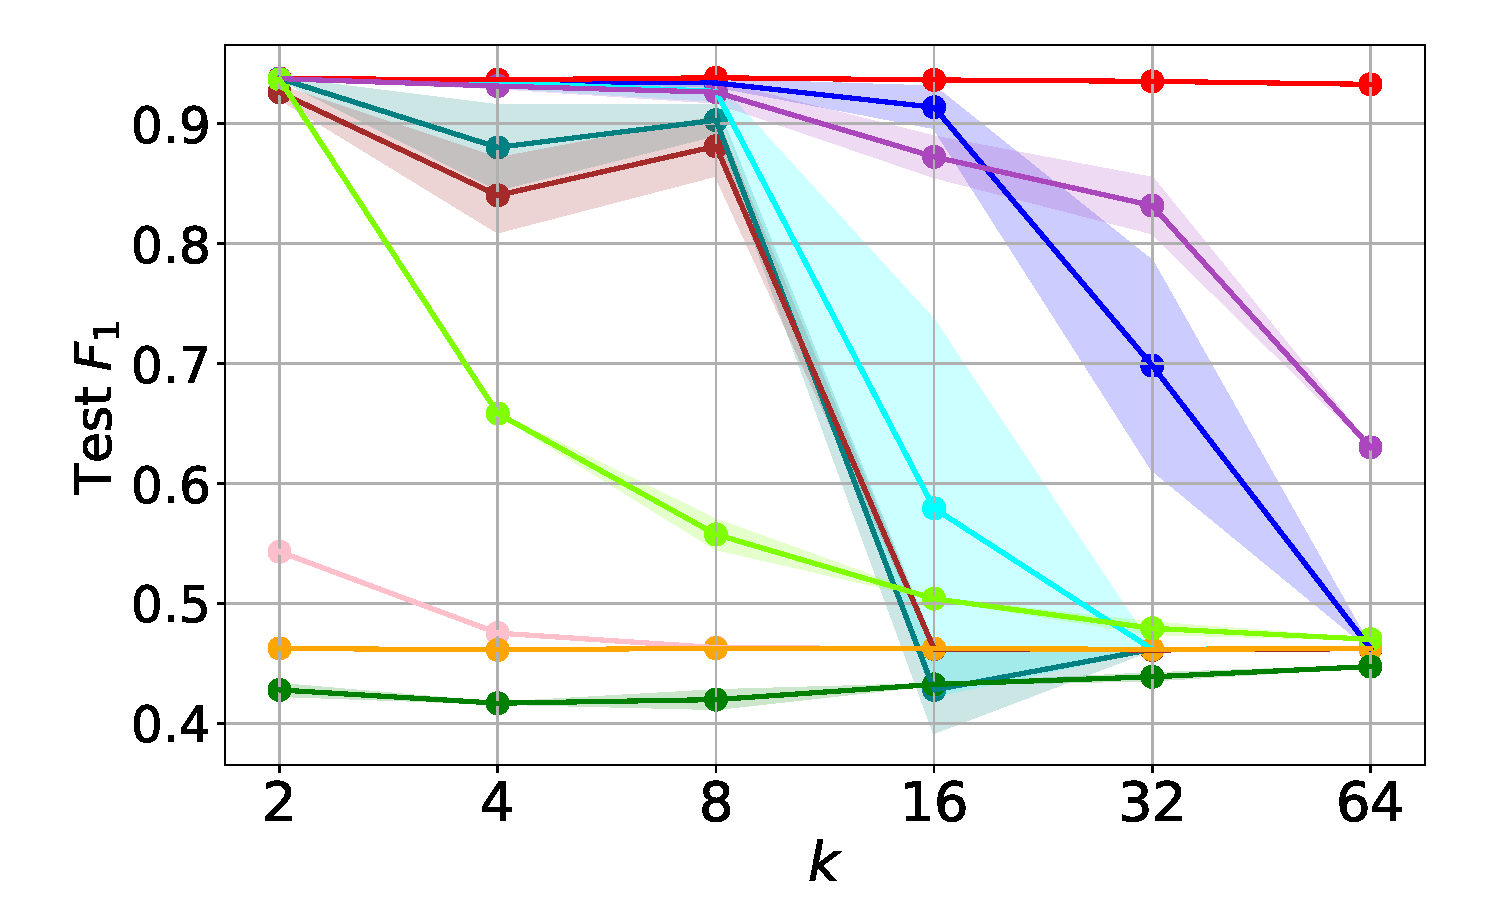
\includegraphics[width=0.35\linewidth]{figs/periodicity/sbm_sto/V2/(0.9, 0.01)(k, 1)All_test avg_f1.pdf}%
        \hspace{0.5cm}%
        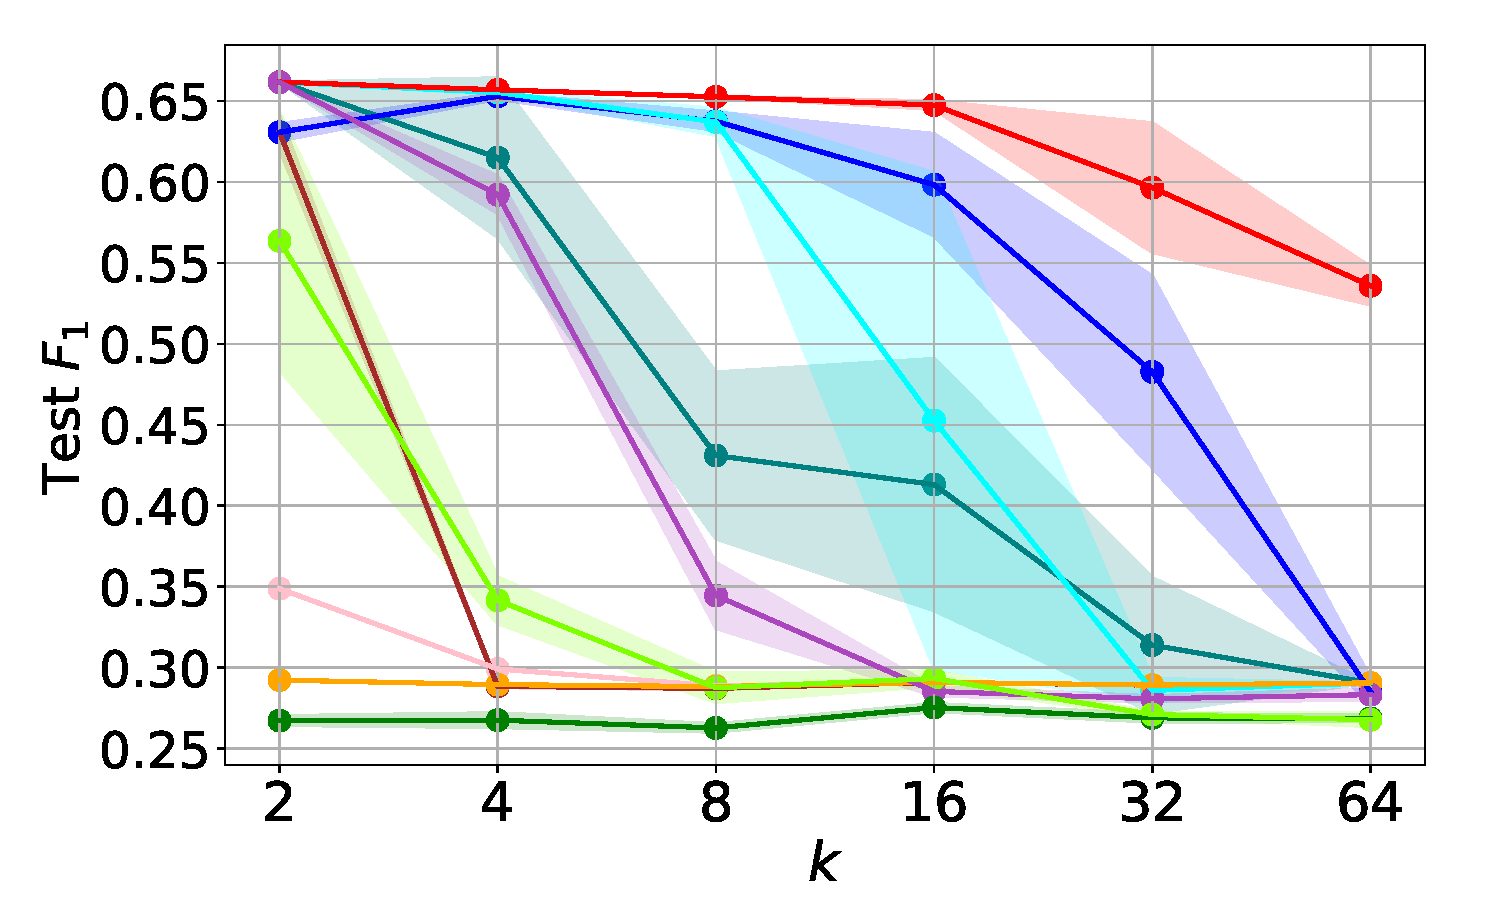
\includegraphics[width=0.35\linewidth]{figs/periodicity/sbm_sto/V2/(0.5, 0.01)(k, 1)All_test avg_f1.pdf}%
        %\hspace{1cm}%
        \raisebox{5mm}{
        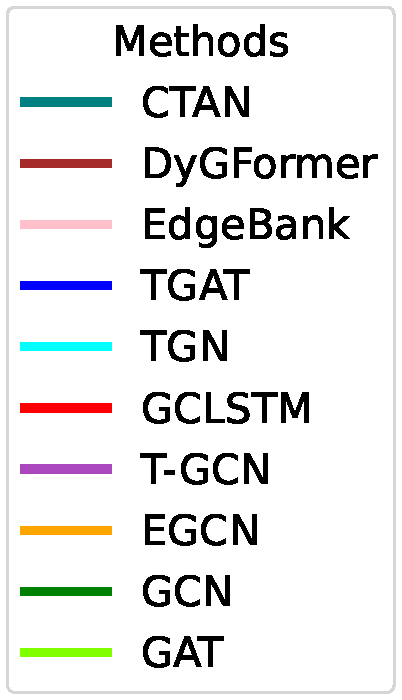
\includegraphics[width=0.08\linewidth]{figs/legends/CTDG DTDG all w edgebank wo persistence.pdf}}
    \caption{ Performance of TGL methods on the stochastic periodicity tasks~$\Psto{k,1}$ for different values of the intra-community edge probability: $p=0.9$ (left) and $p=0.5$ (right).
    % \mh{I don't understand why do we have p=0.5 here? what does it tell that the left plot is not telling us?
    % In text we say
    % "overall, the performance gap between models widens under lower intra-community density (p = 0.5)"
    % Which I don't think is true, at least it's not clearly visible in left and right plot
    % I suggest remove left hand plot or more it to appendix and remove the mentioned sentence.
    % }
    }
    \label{fig:(K,1)_overall_sto}
\end{figure}

